\documentclass[tikz,border=7pt]{standalone}
\usepackage[T1]{fontenc}
\usepackage{lmodern}
\usepackage{helvet}
\renewcommand{\familydefault}{\sfdefault}
\usepackage[table]{xcolor}
\usepackage{tikz}
\usetikzlibrary{arrows.meta,positioning,calc}
\definecolor{ink}{HTML}{163B60}
\definecolor{wash}{HTML}{E4F1FC}
\tikzset{box/.style={draw=ink,rounded corners=3pt,line width=.8pt,minimum height=1cm,align=center,inner sep=8pt},flow/.style={-{Stealth[length=2.5mm]},draw=ink,line width=1pt},font=\sffamily\normalsize,every node/.style={text=ink}}
\begin{document}
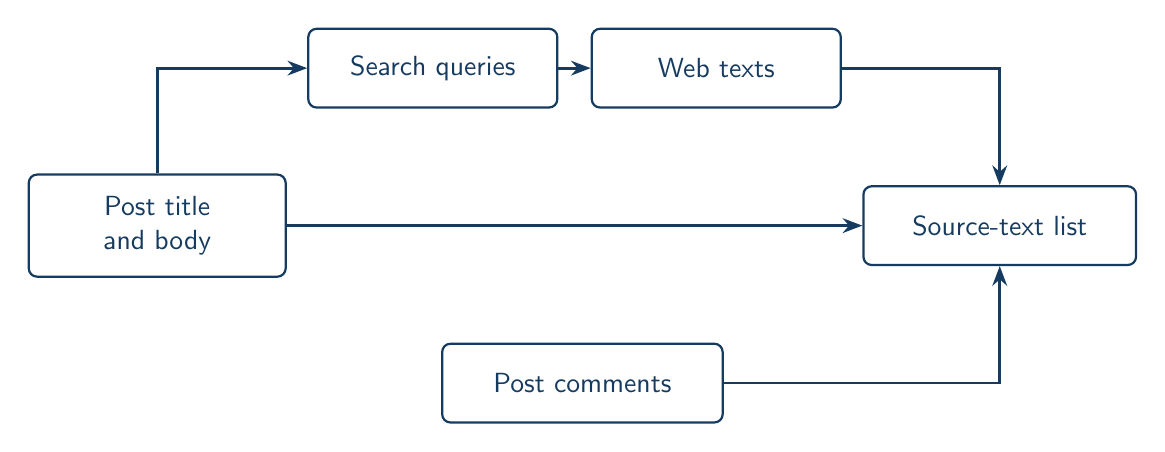
\begin{tikzpicture}
\node[box,text width=2.7cm] (post) at (0,0) {Post title\\and body};
\node[box,text width=2.6cm] (queries) at (3.5,2) {Search queries};
\node[box,text width=2.6cm] (web) at (7.1,2) {Web texts};
\node[box,text width=2.9cm] (texts) at (10.7,0) {Source-text list};
\node[box,text width=3cm] (comments) at (5.4,-2) {Post comments};
\draw[flow] (post.north) |- (queries.west);
\draw[flow] (queries) -- (web);
\draw[flow] (web.east) -| (texts.north);
\draw[flow] (post) -- (texts);
\draw[flow] (comments.east) -| (texts.south);
\end{tikzpicture}
\end{document}
